% Intended LaTeX compiler: lualatex
\documentclass[10pt, svgnames]{beamer}
\usepackage{graphicx}
\usepackage{longtable}
\usepackage{wrapfig}
\usepackage{rotating}
\usepackage[normalem]{ulem}
\usepackage{amsmath}
\usepackage{amssymb}
\usepackage{capt-of}
\usepackage{hyperref}
\usetheme{metropolis}
\author{Sappinandana Akamphon}
\date{\today}
\title{Clutches and Brakes}
\usepackage{booktabs}
\usepackage{pgfplots}
\usepgfplotslibrary{fillbetween}
\institute{Department of Mechanical Engineering, TSE}
\date{}
\AtBeginSection[]{\begin{frame}{Outline}\tableofcontents[currentsection]\end{frame}}
\hypersetup{
 pdfauthor={Sappinandana Akamphon},
 pdftitle={Clutches and Brakes},
 pdfkeywords={},
 pdfsubject={},
 pdfcreator={Emacs 29.0.50 (Org mode 9.6)}, 
 pdflang={English}}
\begin{document}

\maketitle
\begin{frame}{Outline}
\tableofcontents
\end{frame}


\section{Clutches + Brakes}
\label{sec:org75f4af4}

\begin{frame}[label={sec:org9fe8313}]{Clutches and Brakes}
\begin{itemize}
\item Rely on friction to transfer torque
\item Easy to engage/disengage
\end{itemize}
\end{frame}

\begin{frame}[label={sec:org568d27d}]{Clutches vs Brakes}
when engaged

\begin{description}
\item[{Clutches}] \(\omega_{in} = \omega_{out} \neq 0\)
\item[{Brakes}] \(\omega_{in} = \omega_{out} = 0\)
\end{description}
\end{frame}

\begin{frame}[label={sec:orgdd21d84}]{Considerations for Clutch and Brake}
\begin{description}
\item[{Actuating force}] force to engage clutch/brake
\item[{Transmitted torque}] torque through mechanism
\item[{Energy loss}] energy dissipated before mechanism is fully engaged
\item[{Temperature rise}] temperature increase from energy loss
\end{description}
\end{frame}

\section{Types of Clutches and Brakes}
\label{sec:org520d7e1}

\begin{frame}[label={sec:org9e3811c}]{Drum Brakes}
\begin{center}
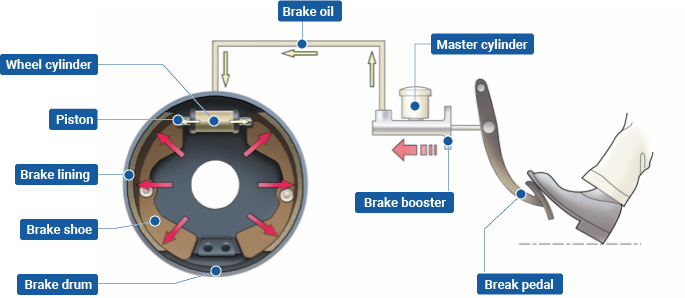
\includegraphics[width=\textwidth]{./pictures/drum-brake.png}
\end{center}
\end{frame}

\begin{frame}[label={sec:orgcb6c0a4}]{Disc Brakes}
\begin{center}
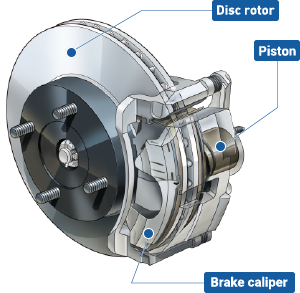
\includegraphics[height=0.9\textheight]{./pictures/disc-brake.png}
\end{center}
\end{frame}

\begin{frame}[label={sec:org600c893}]{Band Brakes}
\begin{center}
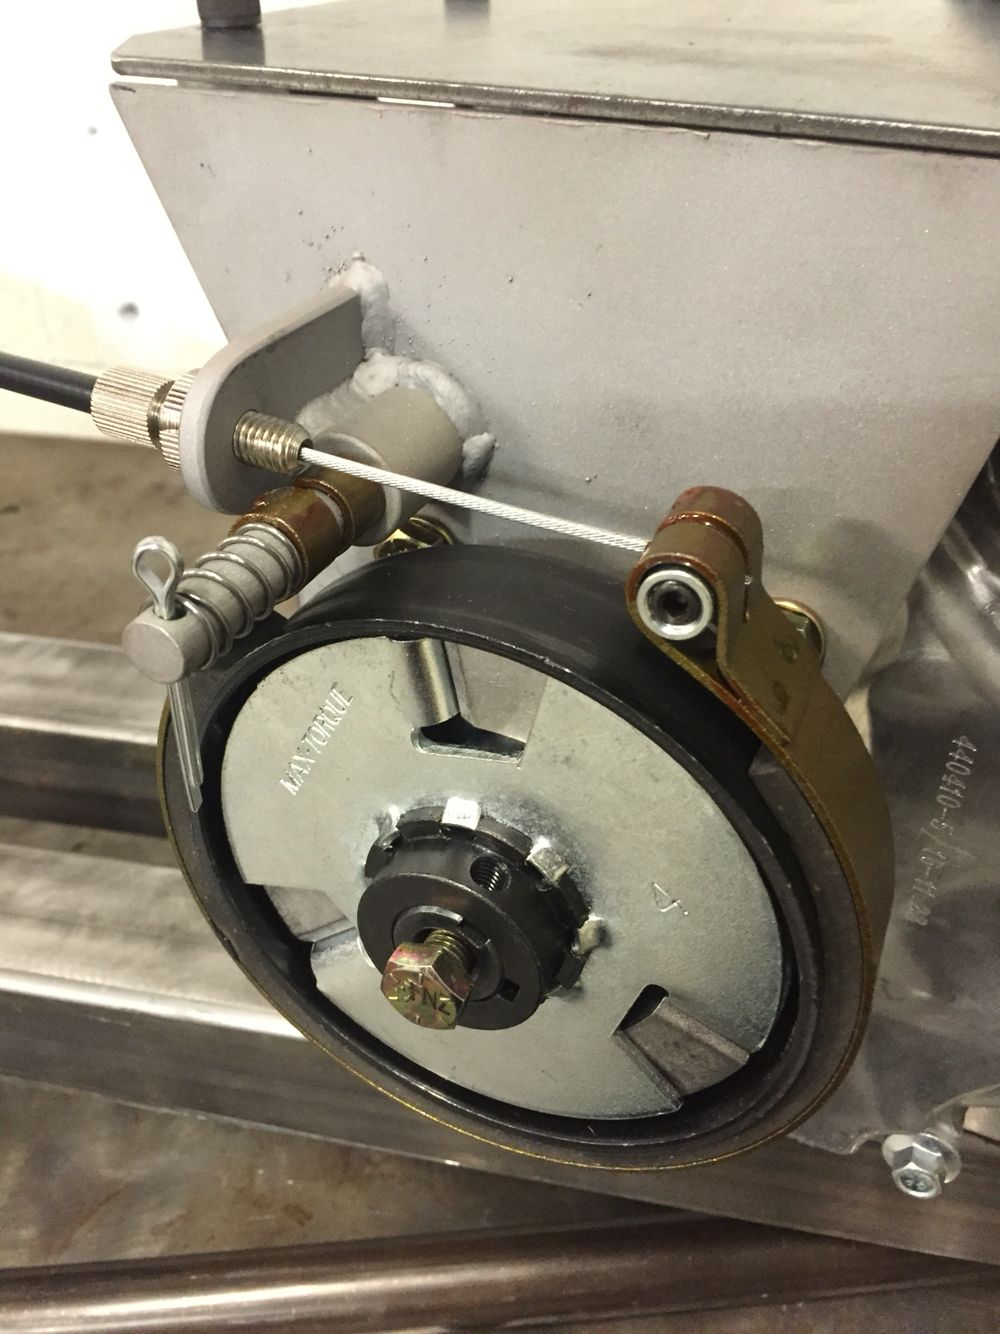
\includegraphics[height=0.9\textheight]{./pictures/band-brake.jpg}
\end{center}
\end{frame}

\section{Brake Linings}
\label{sec:org197949c}

\begin{frame}[label={sec:org519880d}]{Materials}
\begin{center}
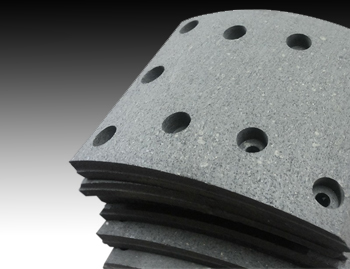
\includegraphics[width=0.3\textwidth]{./pictures/molded-lining.jpg}
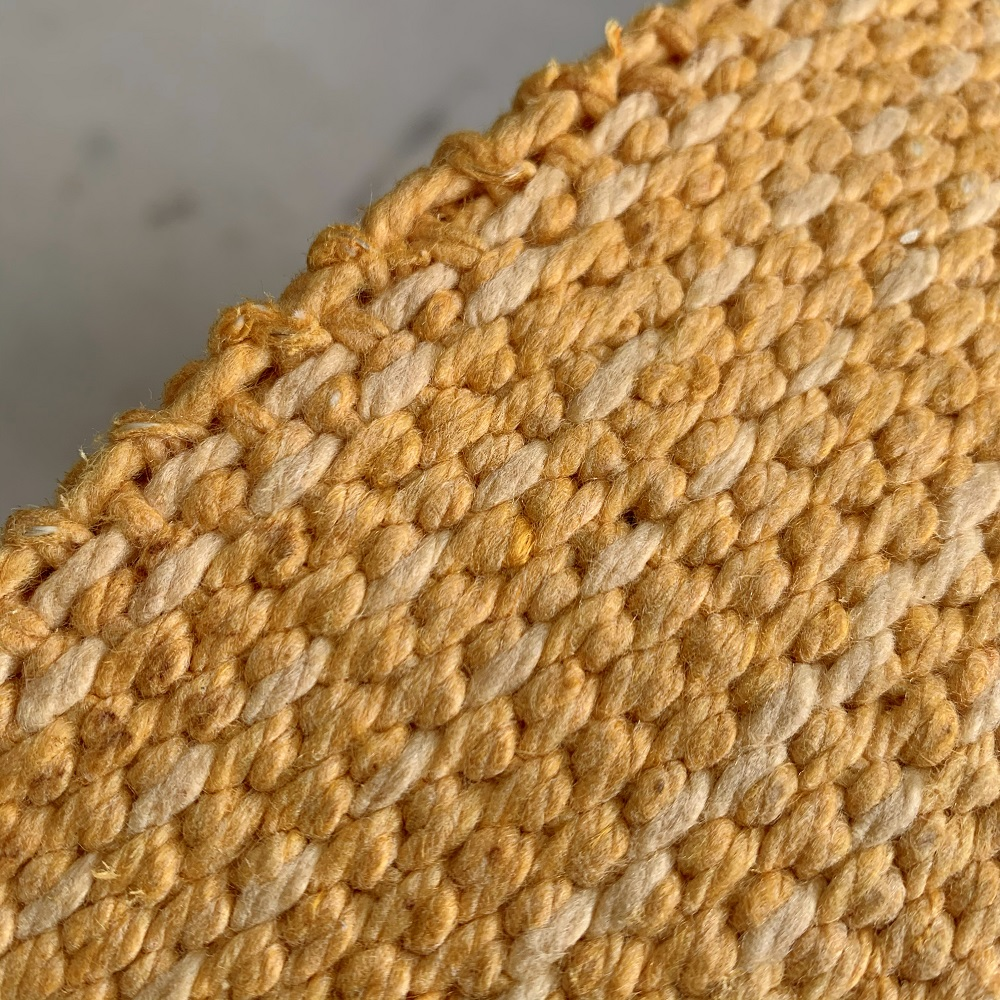
\includegraphics[width=0.3\textwidth]{./pictures/woven-lining.jpg}
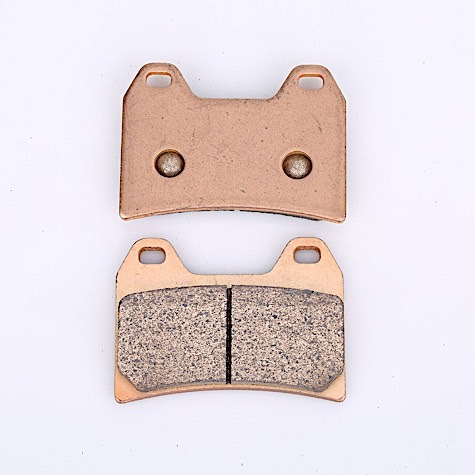
\includegraphics[width=0.3\textwidth]{./pictures/sintered-lining.jpg}
\end{center}

\begin{description}
\item[{Molded}] thermosetting polymer or rubber + heat resistant fibers
\item[{Woven}] fibers + brass or zinc woven into fabric + resin
\item[{Sintered metal}] metal powder + inorganic fillers molded and sintered
\end{description}
\end{frame}

\begin{frame}[label={sec:org18d079f}]{Dry Linings}
\begin{center}
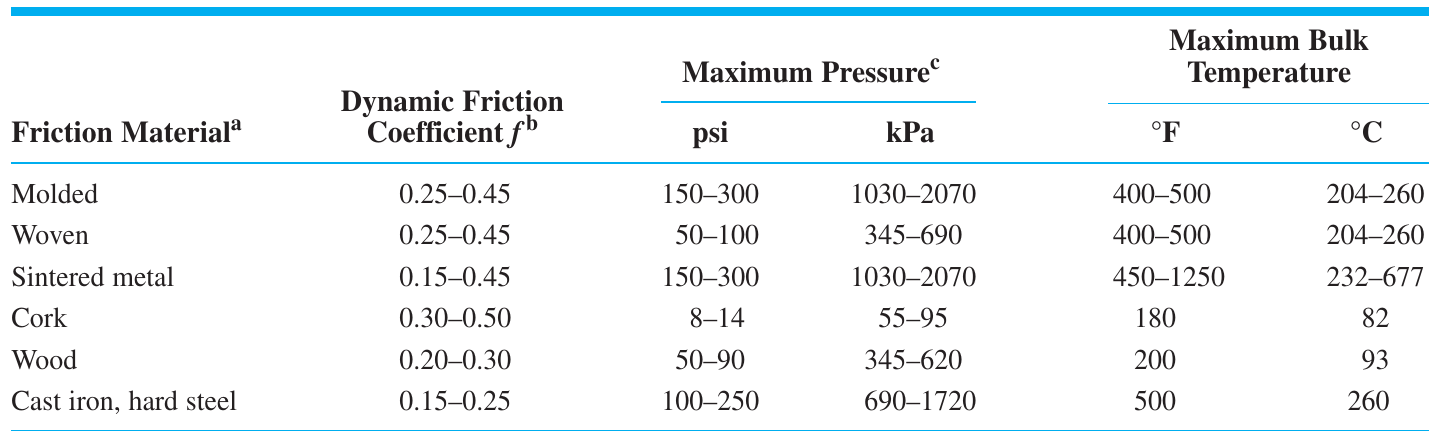
\includegraphics[width=\textwidth]{./pictures/dry-materials.png}
\end{center}
\end{frame}

\begin{frame}[label={sec:orgdec5aa2}]{Wet Linings}
\begin{center}
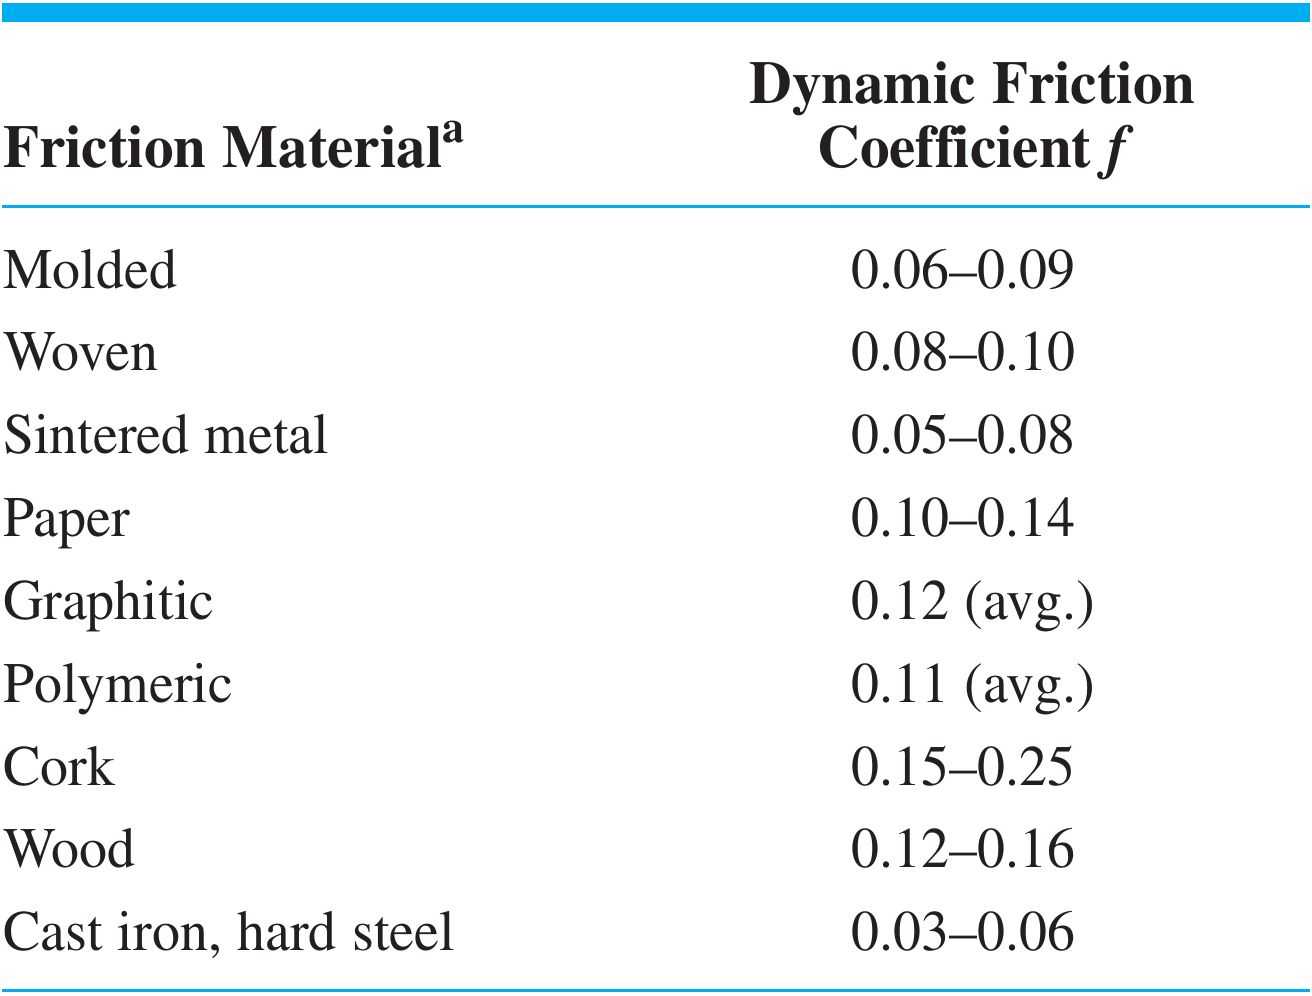
\includegraphics[width=0.8\textwidth]{./pictures/wet-materials.png}
\end{center}
\end{frame}

\section{Drum Brake}
\label{sec:orgcfecb26}

\begin{frame}[label={sec:orgb715448}]{Internal Drum Brake}
\begin{columns}
\begin{column}{0.6\columnwidth}
\begin{center}
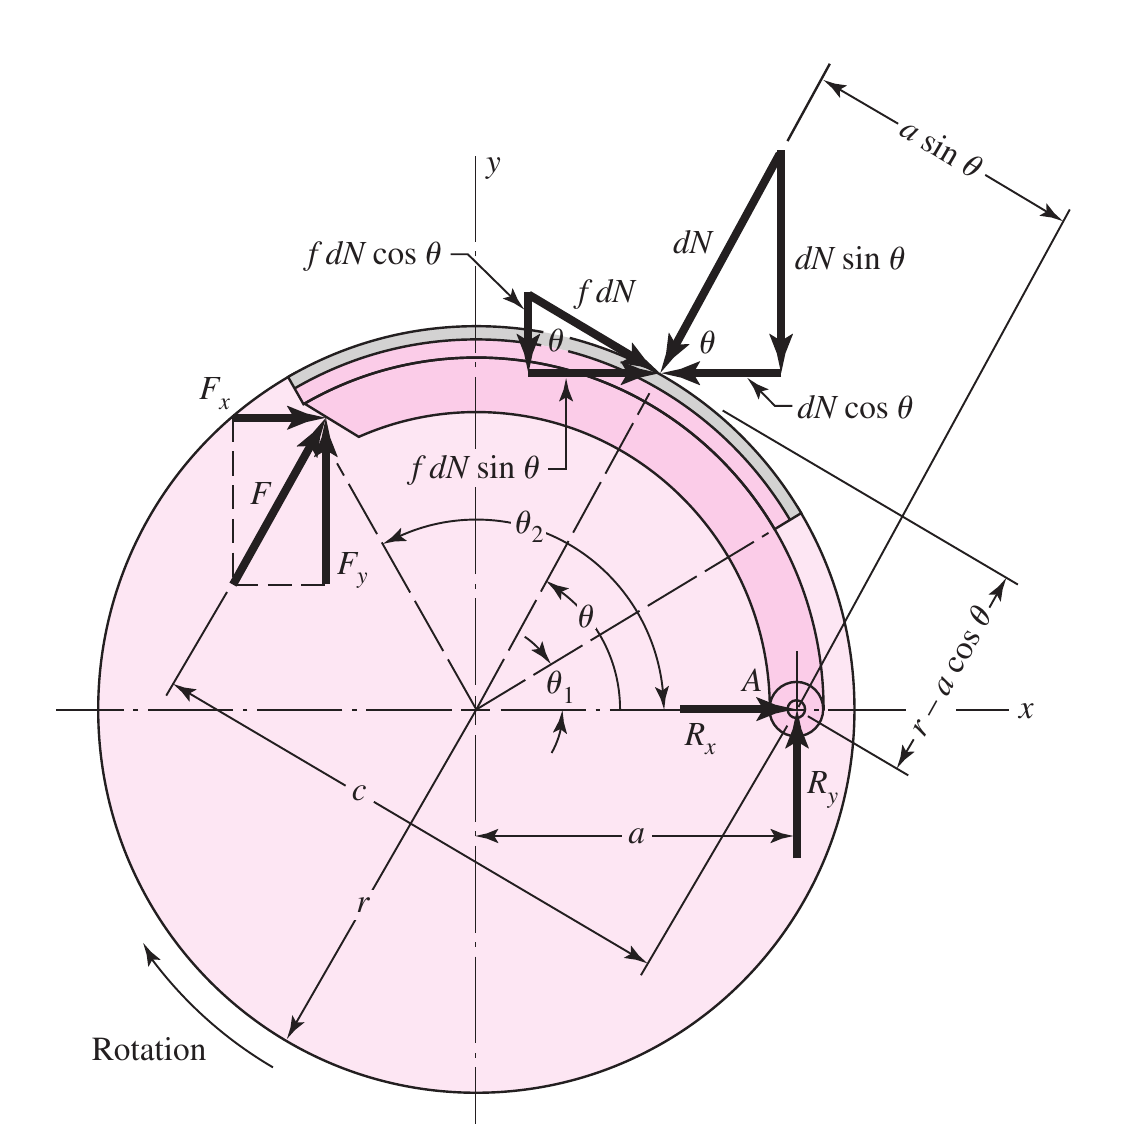
\includegraphics[width=1.1\textwidth]{./pictures/internal-drum-brake.png}
\end{center}
\end{column}

\begin{column}{0.4\columnwidth}
\begin{itemize}
\item Considering moments about \(A\) \(\rightarrow\) 3 moments

\begin{itemize}
\item moment from normal force, \(M_{n}\)
\item moment from friction, \(M_{f}\)
\item moment from actuating force, \(Fc\)
\end{itemize}
\end{itemize}
\end{column}
\end{columns}
\end{frame}

\begin{frame}[label={sec:org2fe167f}]{Pressure Distribution on Drum}
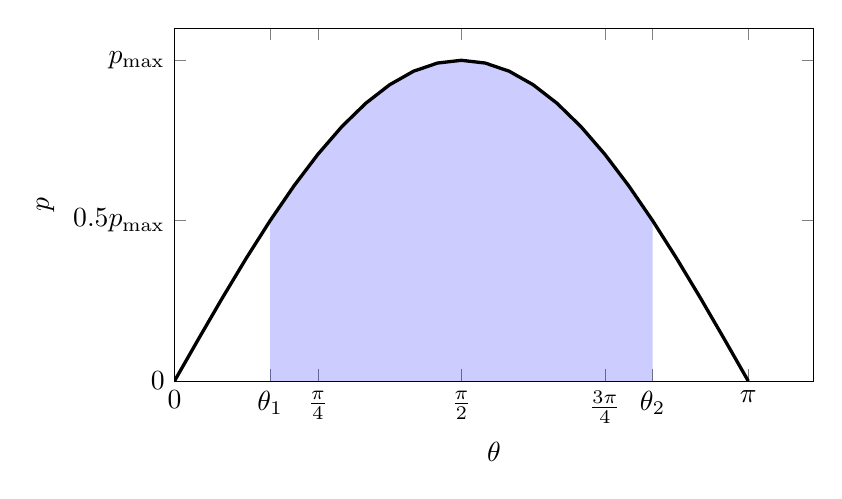
\begin{tikzpicture}
    \begin{axis}[
      width=0.8\textwidth,
      height=.5\textwidth,
      xmin=0,xmax=3.5,
      ymin=0,
      xlabel={$\theta$},
      ylabel={$p$},
      ytick={0,0.5,1},
      yticklabels={0,0.5$p_{\max}$,$p_{\max}$},
      xtick={0,pi/6,pi/4,pi/2,3*pi/4,5*pi/6,pi},
      xticklabels={0,$\theta_{1}$, $\frac{\pi}{4}$, $\frac{\pi}{2}$ , $\frac{3\pi}{4}$,$\theta_{2}$,$\pi$},
      ]
      \addplot [very thick, domain=0:pi, name path=A] {sin(x*180/pi)};
      \addplot [name path=B]{0};
      \addplot[fill=blue, fill opacity=0.2] fill between[of=A and B, soft clip={domain=pi/6:5*pi/6}];
    \end{axis}
  \end{tikzpicture}
\begin{align*}
    p &= \frac{p_{\max}}{(\sin \theta)_{\max}} \sin \theta
\end{align*}

\begin{itemize}
\item \((\sin \theta)_{\max}\) = maximum value of \(\sin\) \(\theta\) for \(\theta_{1} \leqslant \theta \leqslant \theta_{2}\) (not always 1)
\end{itemize}
\end{frame}

\begin{frame}[label={sec:org7fb114f}]{Moment Generated on Drum by Normal Force}
\begin{align*}
    M_n &= \int_{\theta_1}^{\theta_2} dN (a \sin \theta) \\
    dN &= p (r d\theta) b \\
    dN &= \frac{p_{\max} br \sin \theta d\theta}{(\sin \theta)_{\max}} \\
    M_n &= \int_{\theta_1}^{\theta_2} \frac{p_{\max} bra \sin^2 \theta}{(\sin \theta)_{\max}} d\theta \\
        &= \frac{p_{\max} bra}{(\sin \theta)_{\max}} \int_{\theta_1}^{\theta_2} \sin^2 \theta d\theta \\
        &= \frac{p_{\max} bra}{4(\sin \theta)_{\max}} [2(\theta_2 - \theta_1) - \sin 2\theta_2 + \sin 2\theta_1]
\end{align*}
\end{frame}

\begin{frame}[label={sec:org361ceb6}]{Moment Generated on Drum by Friction}
\begin{align*}
    M_f &= \int_{\theta_1}^{\theta_2} \mu dN (r - a \cos \theta) \\
        &= \int_{\theta_1}^{\theta_2} \frac{\mu p_{\max} \sin \theta r d\theta b (r - a \cos \theta)}{(\sin \theta)_{\max}} \\
        &= \frac{\mu p_{\max} br}{(\sin \theta)_{\max}} \left[ r( \cos \theta_1 - \cos \theta_2) + \frac{a}{4}(\cos 2\theta_2 - \cos 2\theta_1) \right]
\end{align*}
\end{frame}

\begin{frame}[label={sec:org3b5ba19}]{Required Actuating Force \(F\)}
\begin{columns}
\begin{column}{0.6\columnwidth}
\begin{center}
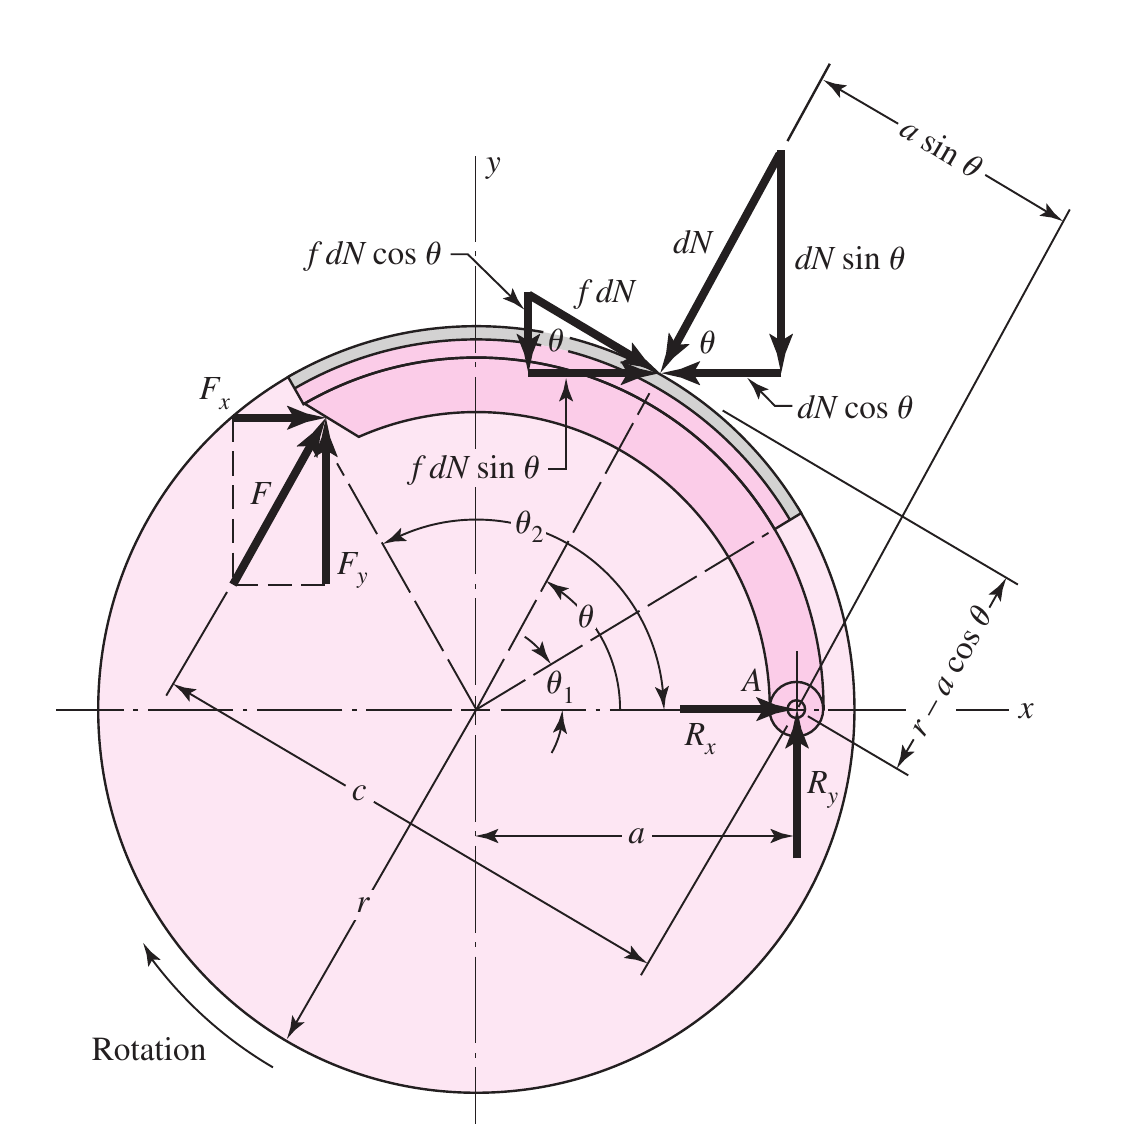
\includegraphics[width=1.1\textwidth]{./pictures/internal-drum-brake.png}
\end{center}
\end{column}

\begin{column}{0.4\columnwidth}
\begin{align*}
    F &= \frac{M_{n} - M_{f}}{c}
\end{align*}

\begin{itemize}
\item If the rotation is reversed, how are the moments changed?
\end{itemize}
\end{column}
\end{columns}
\end{frame}

\begin{frame}[label={sec:orge83a1ef}]{Self-energizing Brake}
\begin{itemize}
\item if \(M_f \geqslant M_n\), the brake is \alert{self-energizing}
\item Moment from friction further presses the shoe against the drum \(\rightarrow\) more braking torque
\item The shoe sticks to the drum \alert{without} actuating force \(F\)
\end{itemize}
\end{frame}

\begin{frame}[label={sec:org3b77192}]{Torque Generated on the Drum}
\begin{align*}
    T &= \int_{\theta_1}^{\theta_2} \mu r dN \\
        &= \frac{\mu r^2 bp_{\max}}{(\sin \theta)_{\max}} \int_{\theta_1}^{\theta_2} \sin \theta d\theta \\
        &= \frac{\mu r^2 bp_{\max}}{(\sin \theta)_{\max}} (-\cos \theta)|_{\theta_1}^{\theta_2} \\
        &= \frac{\mu r^2 bp_{\max}}{(\sin \theta)_{\max}} (\cos \theta_1 - \cos \theta_2) \\
\end{align*}
\end{frame}

\begin{frame}[label={sec:orgb019ca5}]{External Drum Brake}
\begin{center}
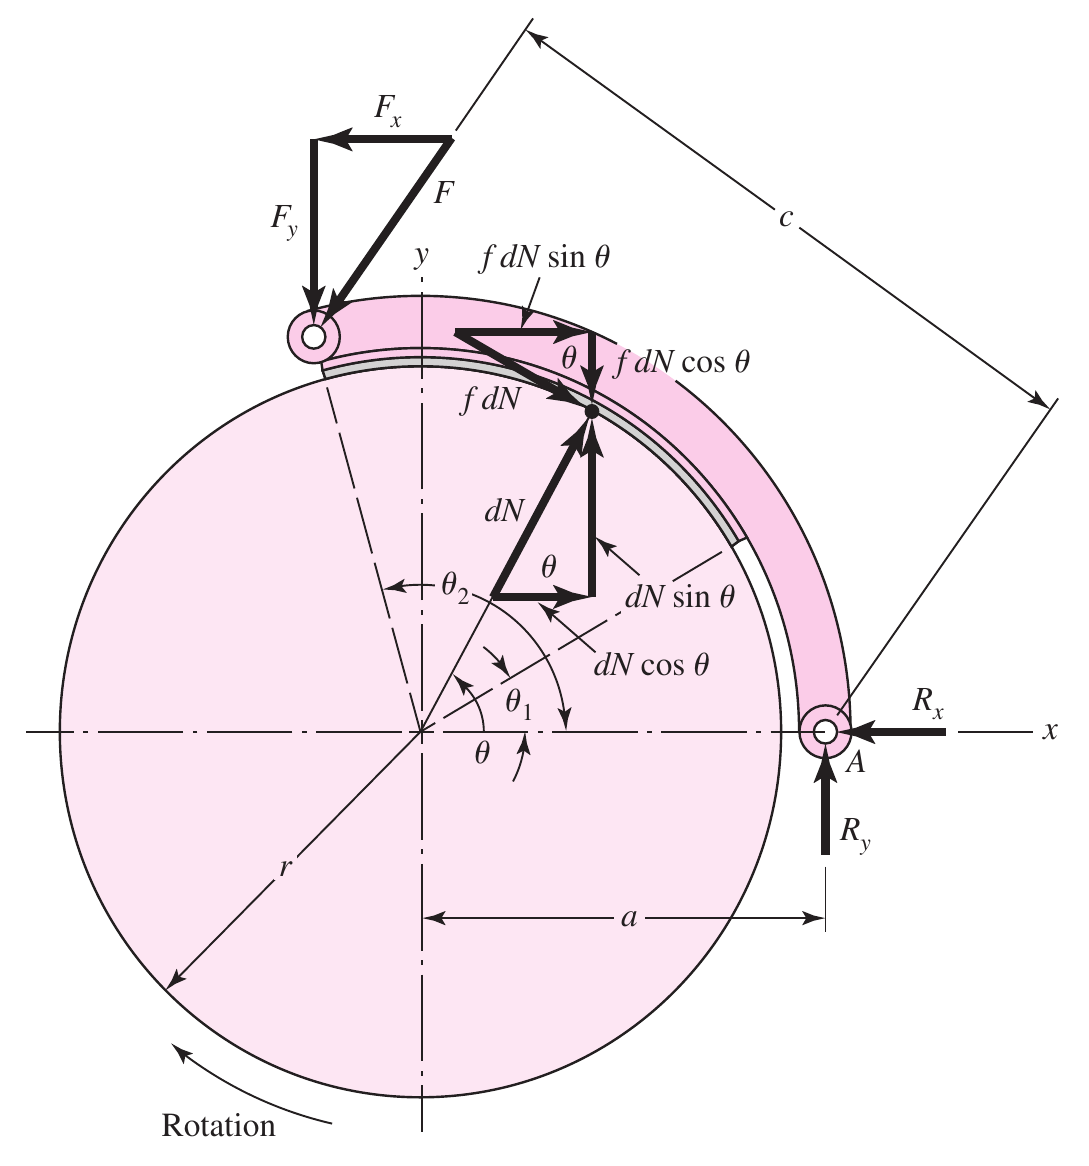
\includegraphics[height=0.9\textheight]{./pictures/external-drum-brake.png}
\end{center}
\end{frame}

\begin{frame}[label={sec:org275e675}]{Required Actuating Force \(F\)}
\begin{itemize}
\item Normal force flip direction
\end{itemize}

\begin{align*}
    F = \frac{M_{n} + M_{f}}{c}
\end{align*}

\begin{itemize}
\item Self-energizing \alert{NOT} possible
\end{itemize}
\end{frame}

\begin{frame}[label={sec:org5bc5b34}]{Torque Generated on the Drum}
\begin{itemize}
\item identical equations to internal drum brake, only need to be careful about the direction of actuating force
\end{itemize}
\end{frame}

\begin{frame}[label={sec:org4bef5d9}]{Example: Braking torque of a drum brake}
\begin{columns}
\begin{column}{0.7\columnwidth}
\begin{center}
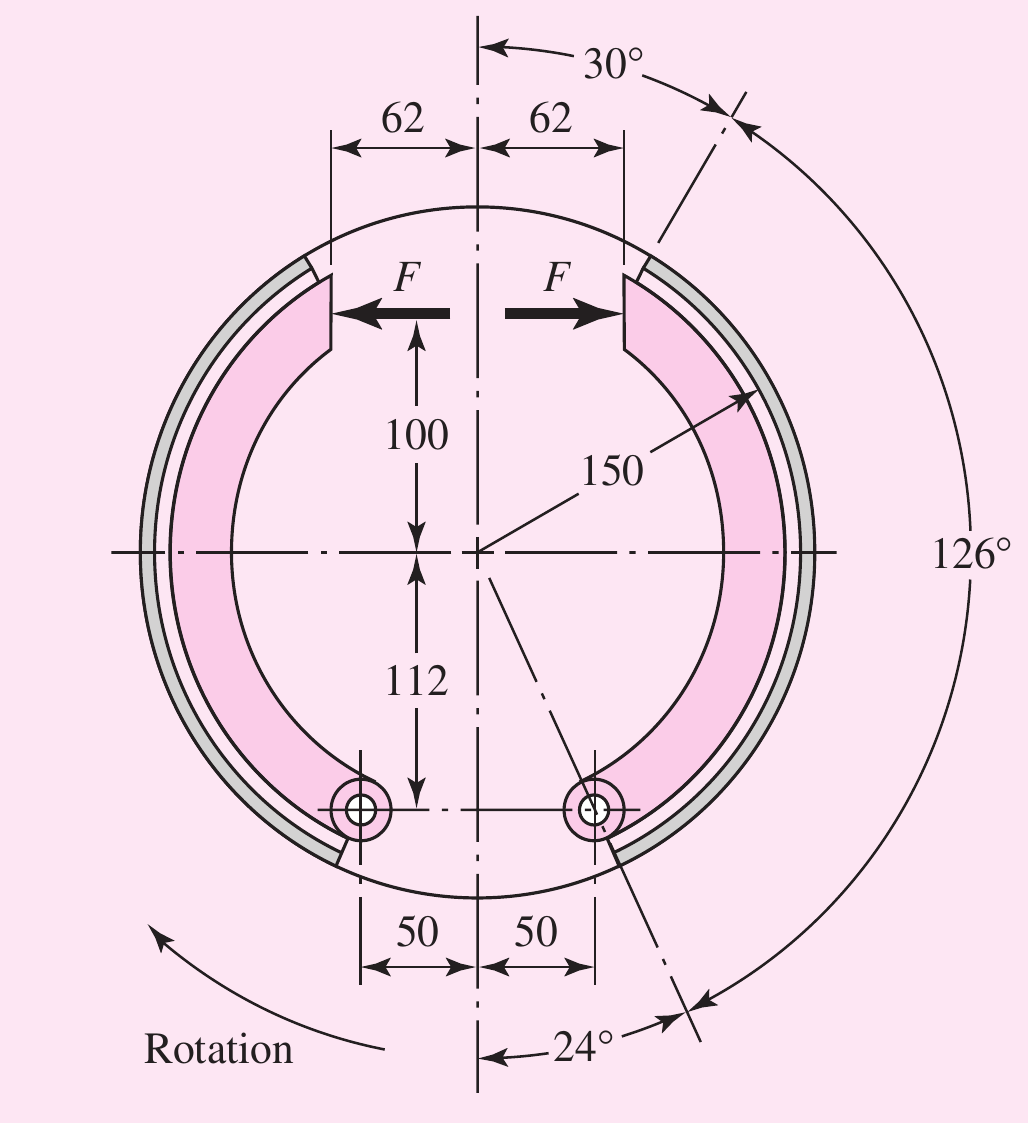
\includegraphics[width=.9\linewidth]{./pictures/drum-example.png}
\end{center}
\end{column}

\begin{column}{0.7\columnwidth}
\begin{itemize}
\item \(F\) = 2000 N
\item \(\mu\) = 0.3
\item \(b\) = 3 cm
\end{itemize}

Determine the braking torque.
\end{column}
\end{columns}
\end{frame}

\begin{frame}[label={sec:org610c761}]{Solution}
First, we must determine \(p_{\max}\) on the right shoe. In this case, \(M_n\) and \(M_f\) go in opposite directions.

\begin{align*}
    Fc &= M_n - M_f \\
    M_n &= \frac{p_{\max} bra}{4(\sin \theta)_{\max}} [2(\theta_2 - \theta_1) - \sin 2\theta_2 + \sin 2\theta_1]
\end{align*}
\end{frame}

\begin{frame}[label={sec:org69e4934}]{Solution}
Let us first find \(M_n\) as a function of \(p_{\max}\)

\begin{align*}
    a &= \sqrt{ 0.112^2 + 0.05^2 } = 0.123 \text{ m} \\
    M_n &= \frac{p_{\max} bra}{4(\sin \theta)_{\max}} [2(\theta_2 - \theta_1) - \sin 2\theta_2 + \sin 2\theta_1] \\
        &= \frac{p_{\max} (0.03)(0.15)(0.123)}{4 (\sin 90^{\circ})} \left[ 2(126^{\circ}(\frac{\pi}{180^{\circ}})) - \sin (2(126^{\circ})) \right] \\
        &= 7.38 \times 10^{-4} p_{\max}
\end{align*}
\end{frame}

\begin{frame}[label={sec:org4182158}]{Solution}
Now find \(M_f\) as a function of \(p_{\max}\)

\begin{align*}
    M_f &= \frac{\mu p_{\max} br}{(\sin \theta)_{\max}} \left[ r( \cos \theta_1 - \cos \theta_2) + \frac{a}{4}(\cos 2\theta_2 - \cos 2\theta_1) \right] \\
        &= \frac{0.3 p_{\max} (0.03)(0.15)}{\sin 90^{\circ}} \left[ (0.15)(\cos 0 - \cos 126^{\circ}) + \right. \\
         & \left. \frac{0.123}{4}(\cos 2(126^{\circ}) - \cos 2(0)) \right] \\
        &= 2.67 \times 10^{-4} p_{\max}
\end{align*}
\end{frame}

\begin{frame}[label={sec:org149e593}]{Solution}
\begin{align*}
    Fc &= M_n - M_f \\
    2000(0.212) &= p_{\max}(7.38 - 2.67) \times 10^{-4} \\
    p_{\max} &= 9.00 \times 10^5 \text{ Pa}
\end{align*}
\end{frame}

\begin{frame}[label={sec:org7f1bd56}]{Solution}
Braking torque of the right shoe is

\begin{align*}
    T_R &= \frac{\mu r^2 bp_{\max}}{(\sin \theta)_{\max}} (\cos \theta_1 - \cos \theta_2) \\
        &= \frac{(0.3)(0.15^2)(0.03)(9.00 \times 10^5)}{1} (\cos 0^{\circ} - \cos 126^{\circ}) \\
        &= 289 \text{ N-m}
\end{align*}
\end{frame}

\begin{frame}[label={sec:orgaf6a0c6}]{Solution}
To calculate braking torque in left shoe, we also must calculate \(p_{\max}\). \(M_n\) and \(M_f\) are now both clockwise.

\begin{align*}
    Fc &= M_n + M_f \\
    2000(0.212) &= (7.38 + 2.67) \times 10^{-4} p_{\max} \\
    p_{\max} &= 4.22 \times 10^5 \text{ Pa}
\end{align*}
\end{frame}

\begin{frame}[label={sec:org91dab69}]{Solution}
Braking torque of the left shoe is

\begin{align*}
    T_L &= \frac{\mu r^2 bp_{\max}}{(\sin \theta)_{\max}} (\cos \theta_1 - \cos \theta_2) \\
        &= \frac{(0.3)(0.15^2)(0.03)(4.22 \times 10^5)}{1} (\cos 0^{\circ} - \cos 126^{\circ}) \\
        &= 136 \text{ N-m}
\end{align*}
\end{frame}

\begin{frame}[label={sec:org4a82141}]{Solution}
Total braking torque is

\begin{align*}
    T &= T_L + T_R \\
        &= 289 + 136 = 425 \text{ N-m}
\end{align*}
\end{frame}

\section{Band Brakes}
\label{sec:org4867a38}

\begin{frame}[label={sec:org2a2d872}]{Principles of Band Brakes}
\begin{itemize}
\item Rely on friction between band and drum
\item Similar to pulley-belt system
\end{itemize}

\begin{align*}
    T = (F_1 - F_2)r
\end{align*}
\end{frame}

\begin{frame}[label={sec:org533a7b4}]{Belt Tension}
\begin{columns}
\begin{column}{0.7\columnwidth}
\begin{center}
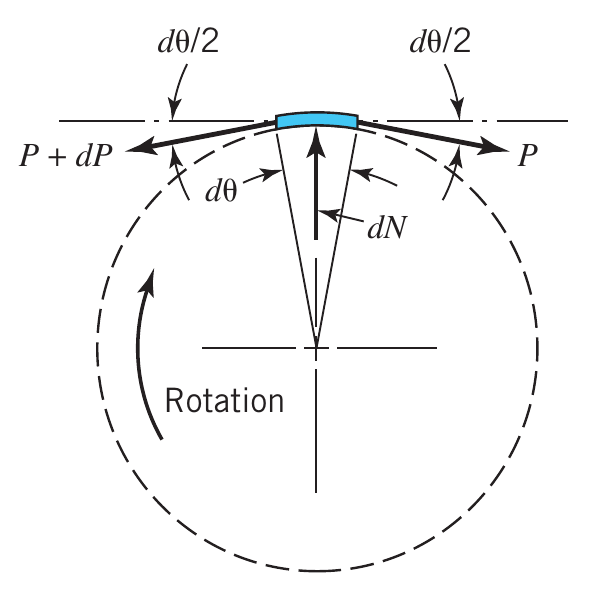
\includegraphics[height=0.8\textheight]{./pictures/band-brake.png}
\end{center}
\end{column}

\begin{column}{0.3\columnwidth}
\begin{align*}
  dF &= \mu dN \\
  dN &= 2(F d\theta/2) = Fd\theta \\
  \frac{dF}{F} &= \mu d\theta \\
  \ln \frac{F_1}{F_2} &= \mu \theta \\
  \frac{F_1}{F_2} &= e^{\mu\theta}
\end{align*}
\end{column}
\end{columns}
\end{frame}

\begin{frame}[label={sec:org137c25c}]{Example: An Exercise Bike}
An exercise bike has an adjustable band brake on the wheel to provide different levels of resistance. What should the slack side belt tension be so that the biker can exercise with \(T\) = 50 N-m. Take \(\theta = 150^{\circ}\) and \(\mu = 0.2\), the bike wheel \(r = 50\) cm.

\begin{center}
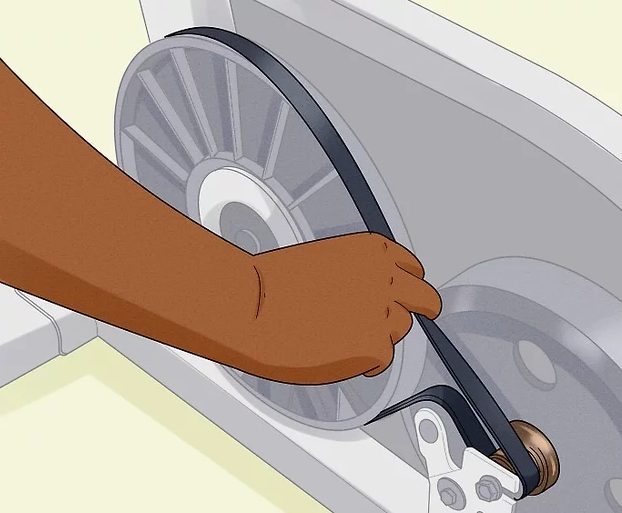
\includegraphics[width=0.6\textwidth]{./pictures/exercise-bike-brake.png}
\end{center}
\end{frame}

\begin{frame}[label={sec:orgc2f89ff}]{Solution}
\begin{align*}
    \frac{F_1}{F_2} &= e^{\mu\theta} \\
    T &= (F_1 - F_2)r \\
    T &= (e^{\mu \theta} - 1) F_2 r \\
    F_2 &= \frac{50}{(e^{0.2(150(\pi/180))}) - 1)(0.5)} \\
        &= 145.3 \text{ N}
\end{align*}
\end{frame}

\section{Disc Clutches and Brakes}
\label{sec:orgf92b37e}

\begin{frame}[label={sec:orga30c674}]{Working Principles}
\begin{center}
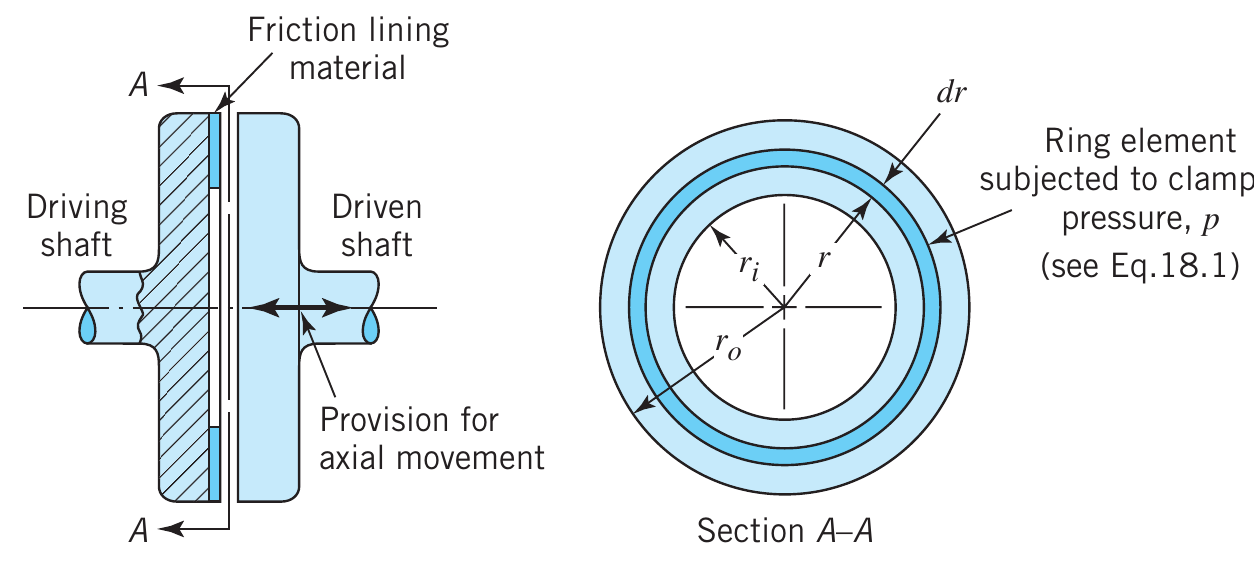
\includegraphics[width=\textwidth]{./pictures/disc-brake-components.png}
\end{center}
\end{frame}

\begin{frame}[label={sec:org2145167}]{Pressure Distribution}
\begin{itemize}
\item New disc is flat, resulting in uniform pressure
\item Outer area wears faster because of higher velocity
\item After a while, pressure is no longer uniform, but wear becomes uniform
\end{itemize}
\end{frame}

\begin{frame}[label={sec:org883ff3f}]{Torque Calculation}
\begin{enumerate}
\item Uniform pressure: new disc
\item Uniform wear: old disc
\end{enumerate}
\end{frame}

\begin{frame}[label={sec:orgbe74e12}]{Torque Calculation: Uniform Pressure}
\begin{align*}
    dF &= p dA \\
    dT &= \mu rdF = \mu r p dA \\
    T &= \int_{r_i}^{r_o} \int_0^{2\pi} \mu r p (rdrd\theta) \\
        &= \frac{2}{3} \mu \pi p \left( r_o^3 - r_i^3 \right)
\end{align*}

\begin{itemize}
\item For \(n\) identical discs
\begin{align*}
T &= \frac{2}{3} n \mu \pi p \left( r_o^3 - r_i^3 \right)
\end{align*}
\end{itemize}
\end{frame}

\begin{frame}[label={sec:orgd5d1869}]{Required Actuating Force for Uniform Pressure}
\begin{center}
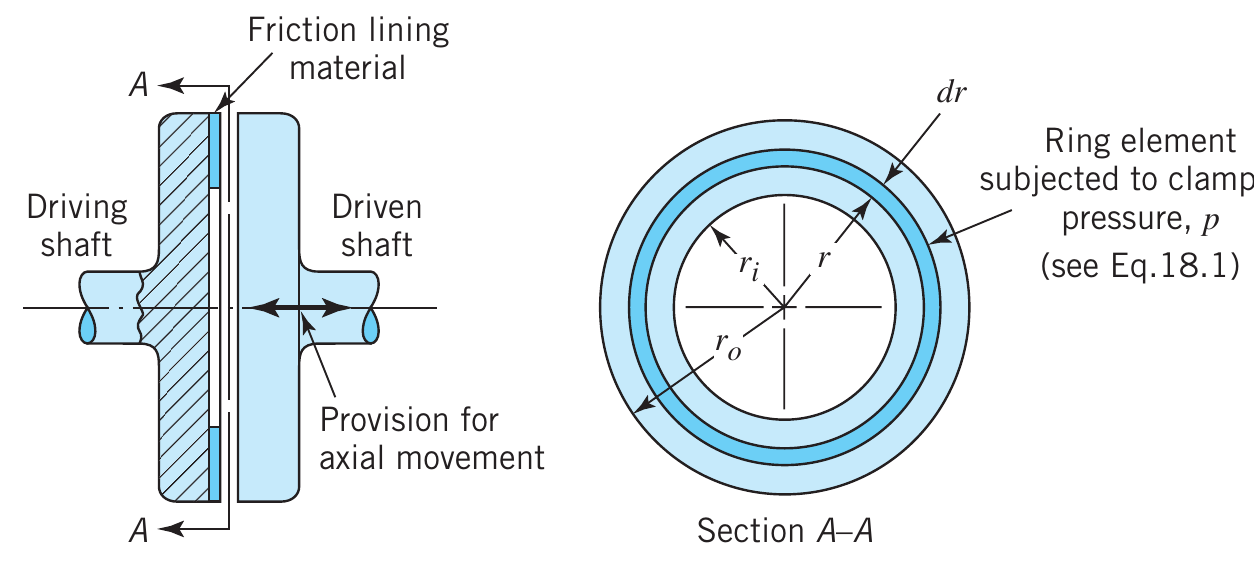
\includegraphics[width=.9\linewidth]{./pictures/disc-brake-components.png}
\end{center}

\begin{align*}
  F &= pA \\
  &= p n \pi \left( r_{o}^{2} - r_{i}^{2} \right)
\end{align*}
\end{frame}

\begin{frame}[label={sec:org306ac0c}]{Uniform Pressure (cont.)}
\begin{itemize}
\item Substitute into \(p = F / n \pi (r_o^2 - r_i^2)\) into \(T\) equation
\end{itemize}

\begin{align*}
T &= \frac{2}{3} n \mu \pi p \left( r_o^3 - r_i^3 \right) \\
&= \frac{2}{3} n \mu \pi \left( r_o^3 - r_i^3 \right) \frac{F}{n \pi (r_o^2 - r_i^2)} \\
&= \frac{2\mu F \left( r_o^3 - r_i^3 \right)}{3 \left( r_o^2 - r_i^2 \right)}
\end{align*}
\end{frame}

\begin{frame}[label={sec:org1eb312b}]{Uniform Rate of Wear}
\begin{itemize}
\item Rate of Wear \(\propto\) Friction Work Rate

$$ pr = C $$

\item Max pressure occurs at inside radius, hence the constant is

$$ pr = C = p_{\max}r_i $$
\end{itemize}
\end{frame}

\begin{frame}[label={sec:orgf06445e}]{Required Actuating Force: Uniform Wear}
\begin{align*}
    dF &= pdA = prdrd\theta \\
     F &= p_{\max} r_{i} \int_{r_{i}}^{r_{o}} \int_{0}^{2\pi} dr d\theta \\
       &= 2p_{\max} r_{i} \pi(r_{o} - r_{i})
\end{align*}

\begin{itemize}
\item For \(n\) parallel discs

\begin{align*}
  F = 2np_{\max}r_{i} \pi(r_{o} - r_{i})
\end{align*}
\end{itemize}
\end{frame}

\begin{frame}[label={sec:org9aed64d}]{Torque Calculation: Uniform Wear}
\begin{align*}
    dF &= pdA \\
    dT &= \mu r dF = \mu r p dA = \mu p_{\max} r_i dA \\
    T &= p_{\max} r_i \int_{r_i}^{r_o} \int_0^{2\pi} r dr d\theta \\
        &= \mu \pi p_{\max} r_i \left( r_o^2 - r_i^2 \right)
\end{align*}

\begin{itemize}
\item For \(n\) parallel discs

$$ T = \mu \pi np_{\max} r_i \left( r_o^2 - r_i^2 \right) $$
\end{itemize}
\end{frame}

\begin{frame}[label={sec:org5de2a2f}]{Torque Calculation: Uniform Wear (cont)}
\begin{itemize}
\item Taking into account actuating force by substituting \(p_{\max}r_{i} = F / 2n \pi (r_{o} - r_{i})\) in \(T\)

\begin{align*}
  T &= \mu \pi np_{\max} r_i \left( r_o^2 - r_i^2 \right) \\
    &= \mu \pi n \left( r_o^2 - r_i^2 \right) \frac{F}{2n \pi (r_{o} - r_{i})} \\
    &= \mu F \left( \frac{r_{o} + r_{i}}{2} \right)
\end{align*}
\end{itemize}
\end{frame}

\begin{frame}[label={sec:orgb47b44b}]{Usual Guideline for Disc Brakes/Clutches}
\begin{enumerate}
\item \(0.45r_o < r_i < 0.8r_o\)
\item Use uniform wear rate, unless for short-term application
\end{enumerate}
\end{frame}

\begin{frame}[label={sec:org078c82c}]{Example: Automotive Clutch}
Design a wet clutch to transfer the torque of 100 N-m using the material with \(\mu\) = 0.08 and \(p_{\max}\) = 1500 kPa. Space requirements only allow \(r_o \leqslant\) 60 mm. Determine the inner diameter and number of parallel discs.
\end{frame}

\begin{frame}[label={sec:org6322ad8}]{Solution}
\begin{itemize}
\item Take \(r_{i} = 0.5r_{o}\) = 30 mm
\end{itemize}

\begin{align*}
    n &= \frac{T}{\left[ \mu \pi p_{\max} r_i \left( r_o^2 - r_i^2 \right) \right]} \\
        &= \frac{100}{\left[ (0.08)\pi(1500 \times 10^3)(0.03) \left( 0.06^2 - 0.03^2 \right) \right]}
\end{align*}

\(N\) = 4 and \(d_i = 2r_i\) = 60 mm
\end{frame}

\begin{frame}[label={sec:orga247d04}]{Drum Brakes vs Disc Brakes}
\begin{center}
\begin{tabular}{p{5cm}p{5cm}}
\toprule
Drum & Disc\\
\midrule
self-energizing possible & no self-energizing\\
\midrule
very sensitive to \(\mu\) & less sensitive to \(\mu\)\\
\midrule
requires larger force once \(\mu\) goes down & well-designed caliper compensate for wear and exert constant pressure\\
\bottomrule
\end{tabular}
\end{center}
\end{frame}
\end{document}
